\subsection{CRUD Interface}

This section presents the CRUD interface implemented for managing game records in the Steam Store Management application.
The interface is designed for the \texttt{GAME} table, which stores the main information of each game, including title, base price, release date, system requirements, and developer ID.

The CRUD interface is implemented as a dedicated tab named \textit{Add/Edit/Delete} in the application.
It provides a form that allows users to enter game information and perform three basic operations: adding a new game, updating an existing game, and deleting a game.
For update and delete operations, the user enters the target \texttt{game\_id}.
For insert operations, the user provides the required game information, including the developer ID.

\subsubsection{Interface Design}

The interface contains input fields for the main attributes of the \texttt{GAME} table, including \texttt{game\_id}, \texttt{title}, \texttt{base\_price}, \texttt{release\_date}, \texttt{graphics}, \texttt{os}, \texttt{processor}, \texttt{memory}, and \texttt{developer\_id}.
Three buttons are provided for the user to execute CRUD actions: \textit{Add Game}, \textit{Update Game}, and \textit{Delete Game}.
The form is illustrated in Figure~\ref{fig:add-edit-game-table}.

When an action is performed, the frontend sends an HTTP request to the backend server.
The backend then calls the corresponding stored procedure in the MySQL database.
This design allows the application to reuse the database logic implemented earlier in Section 2.1 instead of placing all validation and modification logic directly in the frontend.

\begin{figure}[H]
    \centering
    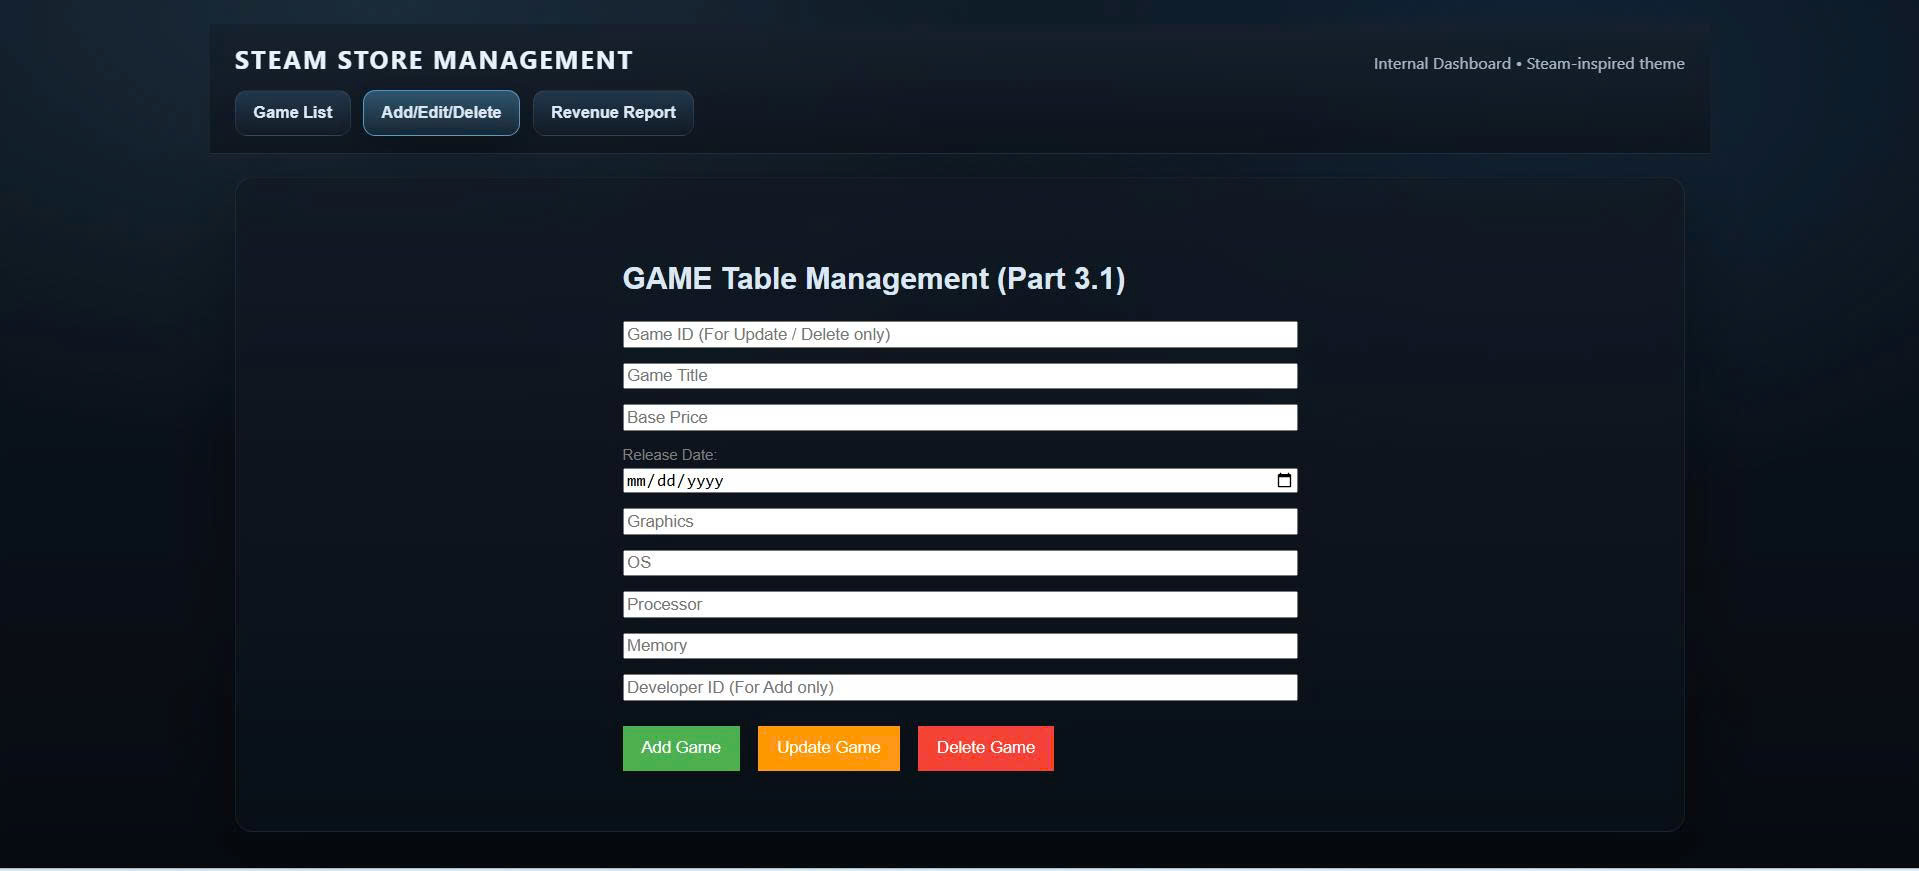
\includegraphics[width=0.9\linewidth]{graphics/Add_Edit_GameTable.jpg}
    \caption{Add/Edit/Delete interface for the \texttt{GAME} table (Part 3.1)}
    \label{fig:add-edit-game-table}
\end{figure}

\begin{table}[H]
\centering
\caption{CRUD operations in the game management interface}
\label{tab:crud-interface-operations}
\begin{tabular}{|l|l|l|}
\hline
\textbf{Operation} & \textbf{Backend Endpoint} & \textbf{Stored Procedure} \\ \hline
Add Game & \texttt{POST /api/games} & \texttt{sp\_InsertGame} \\ \hline
Update Game & \texttt{PUT /api/games/:id} & \texttt{sp\_UpdateGame} \\ \hline
Delete Game & \texttt{DELETE /api/games/:id} & \texttt{sp\_DeleteGame} \\ \hline
\end{tabular}
\end{table}

\subsubsection{Backend Connection}

The backend is implemented using Node.js and Express.
It receives requests from the React frontend and connects to the MySQL database.
For each CRUD operation, the backend does not execute raw insert, update, or delete statements directly.
Instead, it calls the stored procedures \texttt{sp\_InsertGame}, \texttt{sp\_UpdateGame}, and \texttt{sp\_DeleteGame}.

This approach keeps the business rules and validation logic inside the database layer.
If the input data violates a validation rule, the stored procedure returns an error message, and the frontend displays that message to the user.

After a successful CRUD operation, the user can switch to the \textit{Game List} tab to verify that the changes have been correctly persisted in the database.
This list view (Figure~\ref{fig:gamelist-after-crud}) is the same screen described in detail in Section~6.2; it is included here as a verification step that the CRUD interface in this section actually modifies the underlying \texttt{GAME} table through the stored procedures.

\begin{figure}[H]
    \centering
    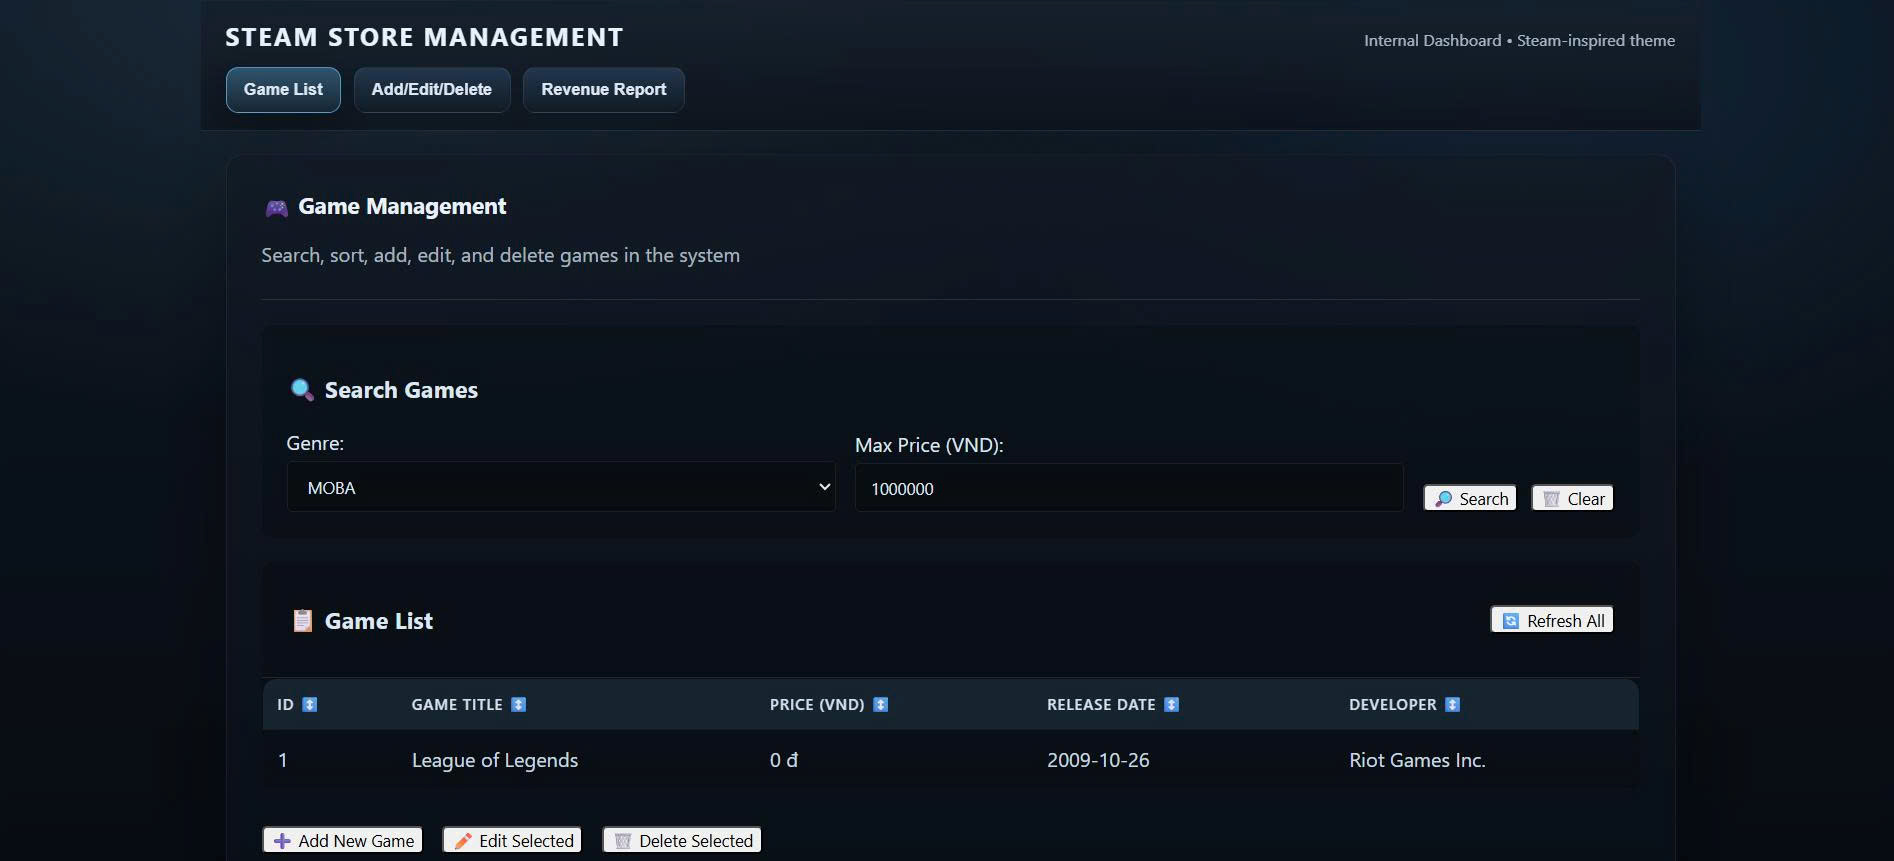
\includegraphics[width=0.9\linewidth]{graphics/GameList.jpg}
    \caption{Game List view used to verify the result of CRUD operations performed in Figure~\ref{fig:add-edit-game-table}}
    \label{fig:gamelist-after-crud}
\end{figure}

The CRUD interface demonstrates that users can manage database records through the application instead of executing SQL statements manually.
It also shows the connection between the frontend, backend API, and database stored procedures.
By using stored procedures for data modification, the application maintains consistent validation rules between the database layer and the user interface.